\begin{center}
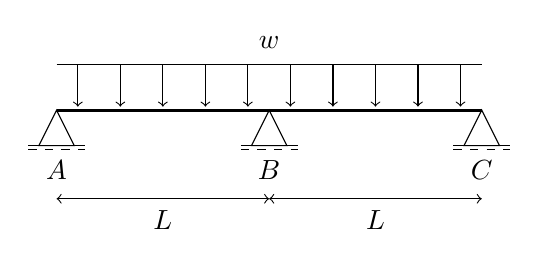
\begin{tikzpicture}[scale=0.9]
\draw[very thick] (0,0) -- (6,0);
\foreach \x in {0.3,0.9,...,5.7} { \draw[->, thin] (\x,0.65) -- (\x,0.05); }
\draw[thin] (0,0.65) -- (6,0.65);
\node at (3,0.95) {$w$};
\foreach \x/\lab in {0/A,3/B,6/C} {
  \draw (\x,0) -- (\x-0.25,-0.5) -- (\x+0.25,-0.5) -- cycle;
  \draw (\x-0.4,-0.5) -- (\x+0.4,-0.5);
  \draw[dashed] (\x-0.4,-0.55) -- (\x+0.4,-0.55);
  \node at (\x,-0.85) {$\lab$};
}
\draw[<->] (0,-1.25) -- (3,-1.25); \node at (1.5,-1.55) {$L$};
\draw[<->] (3,-1.25) -- (6,-1.25); \node at (4.5,-1.55) {$L$};
\end{tikzpicture}

\emph{Figure 1. A beam on three equally spaced supports under a uniform load.}
\end{center}
